\documentclass[12pt,a4paper]{article}

%------------------------------------------------
% Packages
%------------------------------------------------
\usepackage[utf8]{inputenc}
\usepackage{graphicx}
\usepackage{amsmath}
\usepackage{booktabs}
\usepackage{hyperref}
\usepackage{float}
\usepackage{geometry}
\usepackage{caption}
\usepackage{subcaption}
\usepackage{listings}
\usepackage{xcolor}

\geometry{margin=1in}

%------------------------------------------------
% Code style for Python
%------------------------------------------------
\lstset{
language=Python,
basicstyle=\ttfamily\small,
keywordstyle=\color{blue},
stringstyle=\color{red},
commentstyle=\color{green!60!black},
numbers=left,
numberstyle=\tiny,
stepnumber=1,
numbersep=5pt,
frame=single,
breaklines=true
}

%------------------------------------------------
% Title
%------------------------------------------------
\title{\textbf{Machine Learning for Fitness Exercise Recognition}\\
\vspace{0.5cm}
\large Classifying Barbell Exercises Using Wearable Sensor Data}

\author{
Mohammed Eid, Ahmed Hossam, Mohammed Salah
}

\date{\today}

%------------------------------------------------
\begin{document}

\maketitle

%------------------------------------------------
% Abstract
%------------------------------------------------
\begin{abstract}
Wearable sensors have become an important tool for tracking physical activity and improving fitness performance. This project focuses on processing and analyzing accelerometer and gyroscope data collected during gym workouts. The goal is to build a machine learning system capable of classifying barbell exercises and counting repetitions. The workflow includes data preprocessing, visualization, outlier detection, feature engineering, machine learning model training, and repetition counting using signal processing techniques. Several models such as Naive Bayes, Support Vector Machines, Random Forest, and Neural Networks are evaluated to determine the most effective approach for exercise classification.
\end{abstract}

\textbf{Keywords:} Machine Learning, Wearable Sensors, Activity Recognition, Feature Engineering, Time Series Analysis

\newpage
\tableofcontents
\newpage

%------------------------------------------------
\section{Introduction}

\subsection{Background}

The rapid growth of wearable technology has enabled individuals to continuously monitor various aspects of their daily lives. Devices equipped with motion sensors such as accelerometers and gyroscopes allow the collection of detailed movement data in real time. This has led to the emergence of the \textit{Quantified Self} concept, where individuals track personal data related to physical activity, health, and behavior in order to gain insights and improve performance.

In the context of sports and fitness, wearable sensors provide an opportunity to automatically analyze workout activities. By capturing body movement during exercises, it becomes possible to apply machine learning techniques to recognize different physical activities and evaluate performance metrics. Such systems can assist athletes, coaches, and fitness enthusiasts in monitoring exercise quality, preventing injuries, and optimizing training routines.

Recent advances in machine learning and signal processing have made it feasible to extract meaningful information from raw sensor data. By analyzing patterns in accelerometer and gyroscope signals, machine learning models can learn to distinguish between different types of exercises and detect repetitions automatically.

\subsection{Problem Statement}

Tracking gym exercises manually can be time-consuming and error-prone. Many individuals rely on manual counting of repetitions and personal estimation of workout intensity. This approach often leads to inaccurate tracking and limited feedback regarding exercise performance.

The main challenge addressed in this project is the automatic recognition of barbell exercises using data collected from wearable motion sensors. Specifically, the project aims to develop a machine learning pipeline capable of analyzing accelerometer and gyroscope signals to classify different exercises performed during strength training sessions.

Additionally, the system should be able to estimate the number of repetitions performed during each exercise set. Achieving this goal requires several steps, including data preprocessing, visualization, outlier detection, feature engineering, and machine learning model training.

\subsection{Project Objectives}

The main objectives of this project are:

\begin{itemize}

\item Process raw accelerometer and gyroscope sensor data collected during gym workouts.

\item Perform exploratory data analysis and visualization to better understand the characteristics of the motion signals.

\item Detect and remove outliers in the dataset using statistical and machine learning methods.

\item Engineer meaningful features from the raw sensor signals using temporal, frequency, and statistical techniques.

\item Train and evaluate multiple machine learning models to classify different barbell exercises.

\item Develop a custom algorithm capable of automatically counting exercise repetitions based on motion patterns.

\end{itemize}

\subsection{Dataset Overview}

The dataset used in this project was collected using the \textbf{MetaMotion} wearable motion sensor developed by MbientLab. The sensor is capable of measuring motion using an integrated accelerometer and gyroscope. These sensors record movement in three-dimensional space, making them suitable for analyzing physical activities such as weightlifting exercises.

The MetaMotion sensor is small, lightweight, and designed for wearable applications. It can be attached to the body or equipment to capture detailed motion data during workouts.

\begin{figure}[H]
\centering
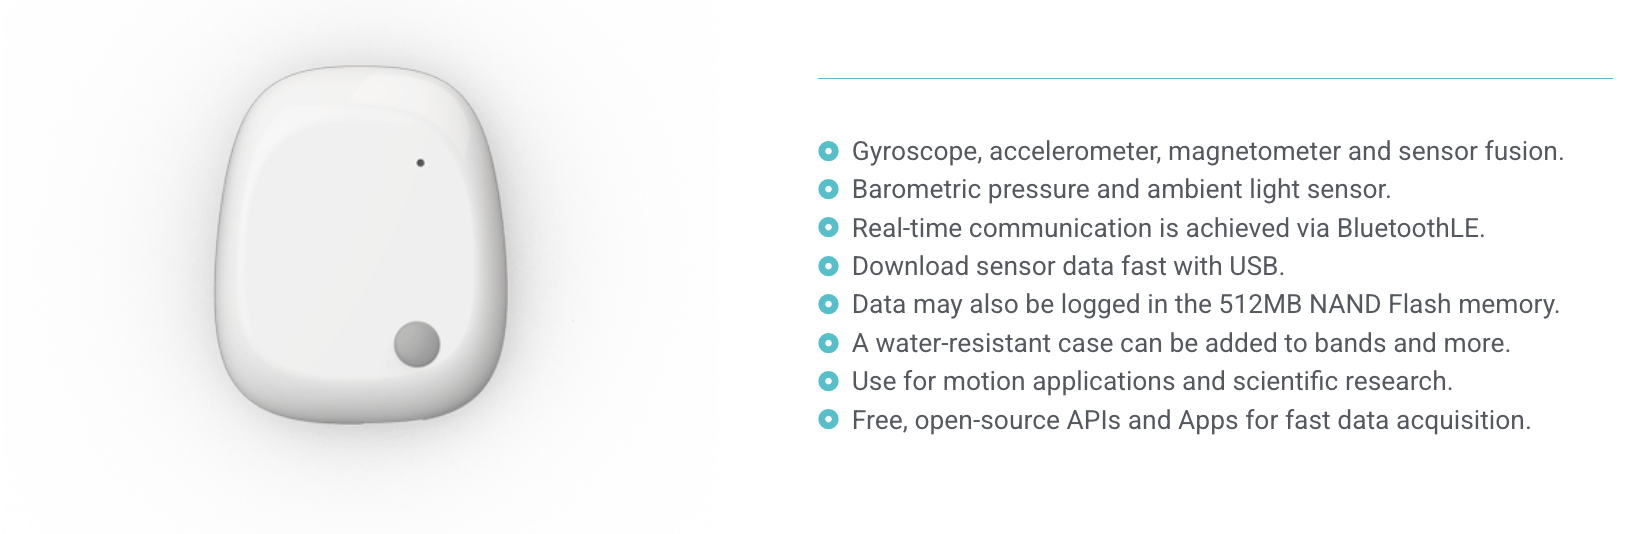
\includegraphics[width=0.9\textwidth]{figures/metamotion_sensor.png}
\caption{MetaMotion wearable motion sensor used for data collection.}
\label{fig:metamotion}
\end{figure}

The dataset contains recordings from multiple participants performing various barbell exercises at different intensity levels. During each workout session, the sensor recorded acceleration and angular velocity along three axes.

The dataset includes the following variables:

\begin{itemize}

\item \textbf{Accelerometer Data:} Acceleration measurements along the X, Y, and Z axes.

\item \textbf{Gyroscope Data:} Angular velocity measurements along the X, Y, and Z axes.

\item \textbf{Participant ID:} Identifier representing the participant performing the exercise.

\item \textbf{Exercise Label:} The type of barbell exercise being performed.

\item \textbf{Exercise Intensity:} The level of effort applied during the exercise (e.g., medium or heavy).

\item \textbf{Set Number:} The specific set within the workout session.

\end{itemize}

An example representation of the recorded motion signals is shown in Figure~\ref{fig:sensor_data_example}.

\begin{figure}[H]
\centering
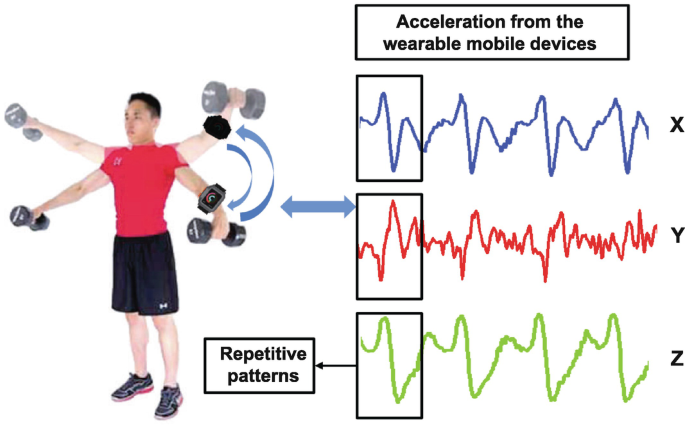
\includegraphics[width=0.85\textwidth]{figures/sensor_data_example.png}
\caption{Example visualization of accelerometer time series signals recorded during an exercise.}
\label{fig:sensor_data_example}
\end{figure}

These motion signals form the basis for the subsequent data analysis and machine learning pipeline developed in this project.
%------------------------------------------------
\section{Related Concepts}

\subsection{Quantified Self}

The \textit{Quantified Self} (QS) movement refers to the practice of collecting and analyzing personal data in order to better understand human behavior, health, and performance. The concept emerged with the rise of wearable technology, mobile devices, and sensor-based systems that allow individuals to continuously monitor different aspects of their daily lives.

In the context of physical activity and fitness, the Quantified Self approach enables individuals to track metrics such as step count, heart rate, sleep quality, and exercise performance. These measurements can provide valuable insights into personal habits and help individuals optimize their lifestyle and training routines.

Machine learning plays an important role in the Quantified Self paradigm. By analyzing large amounts of sensor data collected over time, machine learning models can identify patterns in human movement and automatically recognize different activities. This capability has applications in health monitoring, sports analytics, rehabilitation, and personalized fitness systems.

The project presented in this report follows the Quantified Self approach by analyzing motion data collected from wearable sensors during gym workouts. The goal is to use this data to automatically classify barbell exercises and estimate the number of repetitions performed.

\subsection{Wearable Sensors}

Wearable sensors are small electronic devices designed to be worn on the body in order to collect physiological or motion-related data. These sensors typically contain multiple components such as accelerometers, gyroscopes, magnetometers, and wireless communication modules.

In fitness and sports applications, wearable sensors are used to track body movements and detect physical activities. The data generated by these sensors provides valuable information about motion patterns, which can be analyzed using signal processing and machine learning techniques.

In this project, motion data is collected using a MetaMotion wearable sensor that records both acceleration and rotational movement during exercise.

\begin{figure}[H]
\centering
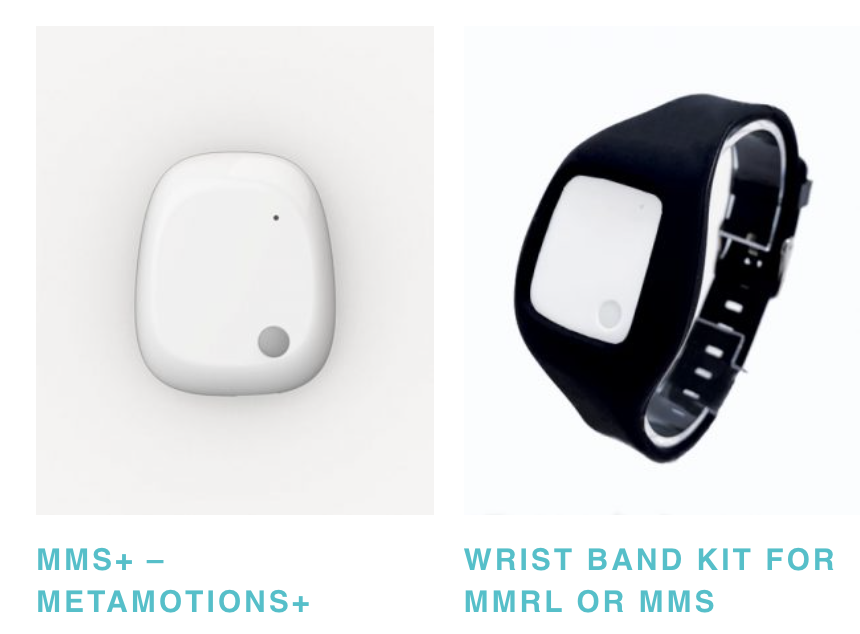
\includegraphics[width=0.6\textwidth]{figures/wearable_sensor_example.png}
\caption{Example of a wearable motion sensor used for activity tracking.}
\label{fig:wearable_sensor}
\end{figure}

Wearable motion sensors typically contain two main types of sensors that are particularly useful for analyzing physical activity: accelerometers and gyroscopes.

\subsubsection{Accelerometer}

An accelerometer is a sensor that measures acceleration forces acting on an object. These forces may be caused by gravity or by movement of the object itself. Accelerometers typically measure acceleration along three orthogonal axes (X, Y, and Z), allowing the detection of movement in three-dimensional space.

In the context of activity recognition, accelerometer data is used to capture patterns of motion such as lifting, walking, or running. For example, during a barbell exercise, the accelerometer can capture the vertical and horizontal movements of the barbell or the athlete's body. These signals can then be analyzed to identify specific exercises and detect repetition cycles.

Accelerometer measurements are usually expressed in units of gravitational acceleration (g), where one g is approximately equal to $9.8 \, m/s^2$.

\begin{figure}[H]
\centering
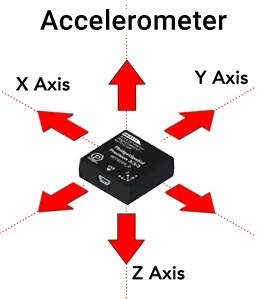
\includegraphics[width=0.4\textwidth]{figures/accelerometer_axes.jpg}
\caption{Accelerometer measurements along three spatial axes (X, Y, Z).}
\label{fig:accelerometer_axes}
\end{figure}

\subsubsection{Gyroscope}

A gyroscope is a sensor that measures angular velocity, which represents the rate of rotation around a particular axis. Similar to accelerometers, gyroscopes measure motion along three axes (X, Y, and Z). However, instead of measuring linear acceleration, they capture rotational movement.

Gyroscope data provides additional information about how an object rotates in space. This is particularly useful when analyzing complex movements such as weightlifting exercises, where both linear and rotational motions occur simultaneously.

For example, during certain barbell exercises, the body or the equipment may rotate slightly during each repetition. The gyroscope can capture these rotational patterns, which helps improve the accuracy of activity recognition models.

Angular velocity is typically measured in degrees per second ($^\circ/s$).

\begin{figure}[H]
\centering
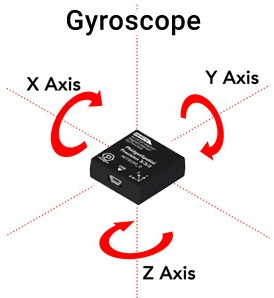
\includegraphics[width=0.4\textwidth]{figures/gyroscope_axes.jpg}
\caption{Gyroscope measurements capturing rotational movement around three axes.}
\label{fig:gyroscope_axes}
\end{figure}

\subsection{Time Series Data}

Sensor measurements collected from wearable devices are recorded sequentially over time. This type of data is known as \textit{time series data}, where each observation is associated with a specific timestamp.

Time series data is commonly encountered in applications such as financial forecasting, weather monitoring, and physiological signal analysis. In the context of wearable sensors, time series data represents continuous recordings of motion signals produced during physical activities.

Analyzing time series data requires specialized techniques because the order and temporal relationships between observations are important. Methods such as filtering, feature extraction, and frequency analysis are often applied to extract meaningful information from these signals.

In this project, accelerometer and gyroscope measurements are recorded at a fixed sampling frequency during workout sessions. These signals form the basis for further data processing steps such as visualization, outlier detection, feature engineering, and machine learning model training.
%------------------------------------------------
\section{Dataset Preparation}

\subsection{Raw Dataset Description}

The raw dataset consists of multiple CSV files containing motion sensor measurements collected during different gym workout sessions. Each exercise session was recorded using a MetaMotion wearable sensor that captures both accelerometer and gyroscope data.

Each CSV file corresponds to a specific sensor type and exercise session. The filenames include useful information such as the participant identifier, the exercise type, and the exercise intensity level. For example, the filename structure encodes:

\begin{itemize}
\item Participant ID
\item Exercise label (e.g., bench, squat, row)
\item Exercise category (e.g., heavy or medium intensity)
\item Sensor type (Accelerometer or Gyroscope)
\end{itemize}

The accelerometer data was recorded at a frequency of 12.5 Hz, while the gyroscope data was recorded at a frequency of 25 Hz. Because the sensors operate at different sampling frequencies, additional preprocessing was required to align the measurements.

\subsection{Reading Raw Data}

Python scripts were used to read all CSV files from the dataset directory and load them into pandas dataframes. The \texttt{glob} library was used to automatically detect all sensor files stored in the raw data folder.

Initially, individual files were loaded to inspect their structure and verify the available columns.

\begin{lstlisting}
import pandas as pd

data = pd.read_csv("sensor_data.csv")
\end{lstlisting}

After inspecting the file structure, a loop was implemented to iterate through all CSV files and load them into two separate dataframes: one for accelerometer measurements and another for gyroscope measurements.

During this step, additional metadata was extracted from the filename, including the participant ID, the exercise label, and the exercise category. These attributes were added as new columns to the dataframe in order to support later analysis and machine learning tasks.

\subsection{Data Cleaning}

Several preprocessing steps were applied to clean and organize the dataset.

First, unnecessary columns such as timestamps in milliseconds, elapsed time, and formatted time strings were removed because they were redundant after creating a proper datetime index.

Next, the epoch timestamp values were converted into Python datetime objects using the pandas \texttt{to\_datetime()} function. These timestamps were then assigned as the dataframe index. Using a datetime index simplifies time-based analysis and enables easier alignment between different sensor measurements.

Finally, accelerometer and gyroscope datasets were combined into unified dataframes containing all recorded sessions.

\subsection{Sensor Data Alignment}

The accelerometer and gyroscope sensors record data at different sampling frequencies (12.5 Hz and 25 Hz respectively). Instead of performing traditional resampling, the datasets were aligned using a time-based merging approach.

The pandas function \texttt{merge\_asof()} was used to match each accelerometer measurement with the closest gyroscope measurement based on their timestamps. This method preserves the temporal structure of the data while efficiently aligning measurements from both sensors.

\begin{lstlisting}
data_merged = pd.merge_asof(
    acc_df.iloc[:,:3].sort_index(),
    gyr_df.sort_index(),
    left_index=True,
    right_index=True
)
\end{lstlisting}

After merging the datasets, the columns were renamed to clearly represent the sensor signals:

\begin{itemize}
\item Accelerometer signals: \texttt{acc\_x}, \texttt{acc\_y}, \texttt{acc\_z}
\item Gyroscope signals: \texttt{gyr\_x}, \texttt{gyr\_y}, \texttt{gyr\_z}
\end{itemize}

Additional metadata columns such as participant ID, exercise label, category, and set number were also retained in the final dataset.

\subsection{Exporting the Processed Dataset}

Once the accelerometer and gyroscope signals were successfully aligned, the processed dataset was saved as a serialized pandas object using the Pickle format. This format allows fast loading in later stages of the machine learning pipeline.

\begin{lstlisting}
data_merged.to_pickle("../../data/interim/01_data_processed.pkl")
\end{lstlisting}

Saving the dataset in this format avoids the need to repeat the preprocessing steps when performing exploratory data analysis, feature engineering, or model training.
%------------------------------------------------
\section{Data Visualization}

Data visualization is an essential step in exploratory data analysis. In this project, visualization is used to understand motion patterns captured by the MetaMotion sensor during different barbell exercises. The accelerometer and gyroscope signals provide detailed information about the movement of the barbell over time. By visualizing these signals, it becomes possible to observe differences between exercises and identify patterns that can later be used for machine learning classification.

\subsection{Visualization Workflow}

The visualization process follows a structured workflow. First, the raw sensor data is loaded and processed to extract relevant metadata such as the participant identifier, exercise label, and training category. These attributes are extracted directly from the filenames of the sensor recordings.

Next, the accelerometer and gyroscope datasets are combined into a single dataset using time-based merging. This ensures that both sensor signals are synchronized according to their timestamps. After merging the datasets, the data is indexed using the timestamp column to allow time-series analysis.

Finally, visualizations are generated using the Matplotlib library. These figures allow us to inspect the sensor signals and explore relationships between exercises and motion patterns.

\subsection{Time Series Visualization}

Time-series visualization is used to analyze how sensor values change over time during exercise execution. Each exercise produces a sequence of accelerometer and gyroscope readings that correspond to the motion of the barbell.

The accelerometer measures linear acceleration in three axes (X, Y, and Z), while the gyroscope measures rotational movement around the same axes. By plotting these signals over time, it becomes possible to observe peaks, oscillations, and repeating patterns that correspond to repetitions of an exercise.

In this project, the accelerometer and gyroscope signals are plotted on separate axes within the same figure to allow clear comparison between linear and rotational motion.

\begin{figure}[H]
\centering
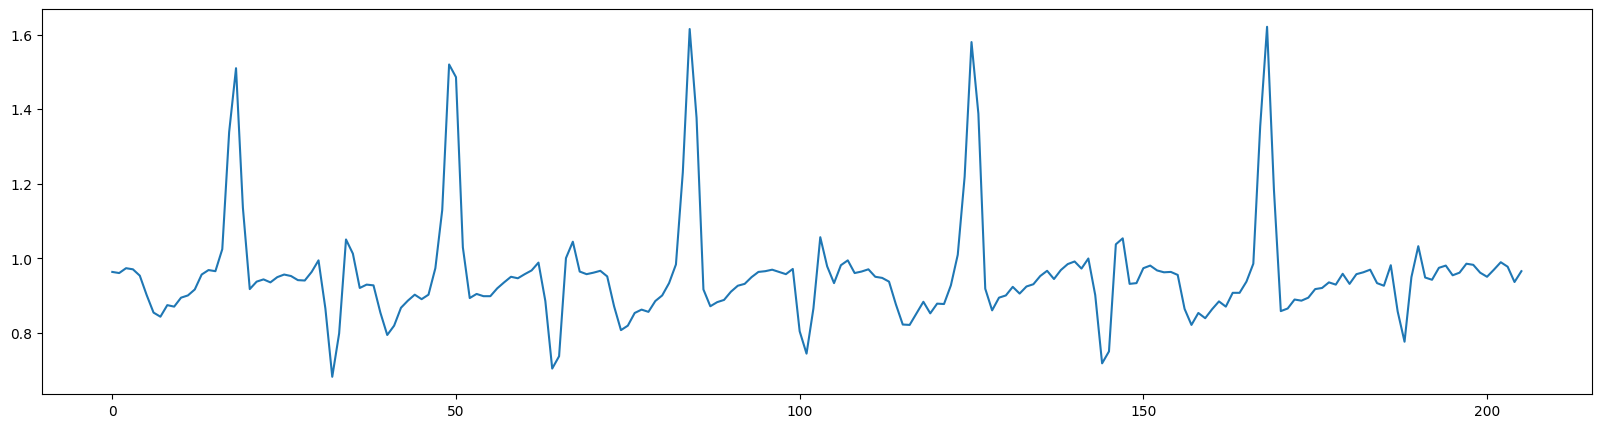
\includegraphics[width=0.95\textwidth]{figures/accelerometer_timeseries.png}
\caption{Example time-series visualization of accelerometer signals during a barbell exercise}
\end{figure}

These plots help reveal how motion intensity changes throughout the exercise and highlight repetitive patterns corresponding to individual repetitions.

\subsection{Exercise Comparison}

Different exercises produce distinct movement patterns in the sensor data. By comparing the time-series plots of different exercises, we can observe clear differences in signal behavior.

For example, exercises such as bench press and overhead press may produce sharp peaks in the acceleration signals due to explosive upward movement. In contrast, squats may show deeper and slower patterns corresponding to the lowering and lifting phases of the movement. These differences can be visually identified when plotting subsets of the sensor data.

\begin{figure}[H]
\centering
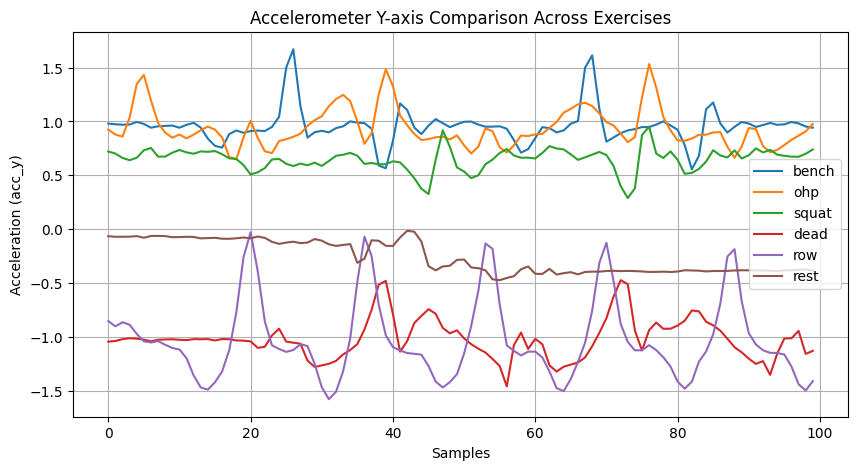
\includegraphics[width=0.95\textwidth]{figures/exercise_comparison.png}
\caption{Comparison of accelerometer signals for different barbell exercises}
\end{figure}

These visual differences demonstrate that each exercise generates a unique motion signature in the sensor data. This observation is crucial for the next stages of the project, where machine learning algorithms will use these patterns to classify exercises automatically.

\subsection{Exporting Visualization Results}

After generating the figures, the plots are exported as high-resolution images. Exporting figures is important when preparing reports or sharing results with others. High-resolution images ensure that visual patterns remain clear and interpretable when included in documentation.

These exported visualizations serve as an important reference for understanding the dataset and validating the preprocessing steps before proceeding to outlier detection, feature engineering, and machine learning modeling.
%------------------------------------------------
\section{Outlier Detection}

In this stage of the project, we detect and remove extreme values from the sensor dataset. 
Outliers are observations that deviate significantly from the majority of the data and may introduce noise or negatively affect machine learning models. 
To identify such values, multiple statistical and machine learning techniques were applied to the accelerometer and gyroscope sensor data.

\subsection{Outliers}

Outliers are extreme values in a dataset that are much higher or lower than the majority of the observations. 
They can appear due to measurement errors, sensor noise, or unusual behavior in the recorded activity. 
In the context of this fitness tracking dataset, outliers may occur due to irregular movements or sensor inaccuracies. 
Identifying and handling these values is important because they can distort statistical measures and reduce model performance.

\subsection{IQR Method}

The Interquartile Range (IQR) method is a statistical technique used to detect outliers based on the distribution of the data. 
It relies on the first quartile ($Q1$) and the third quartile ($Q3$) of a dataset. The IQR is calculated as:

\[
IQR = Q3 - Q1
\]

Outliers are then defined as values outside the following bounds:

\[
\text{Lower Bound} = Q1 - 1.5 \times IQR
\]

\[
\text{Upper Bound} = Q3 + 1.5 \times IQR
\]

Any observation that falls outside these limits is considered an outlier. 
In this project, the IQR method was applied to each sensor column individually (e.g., accelerometer and gyroscope axes) to identify extreme values.

\begin{figure}[H]
\centering
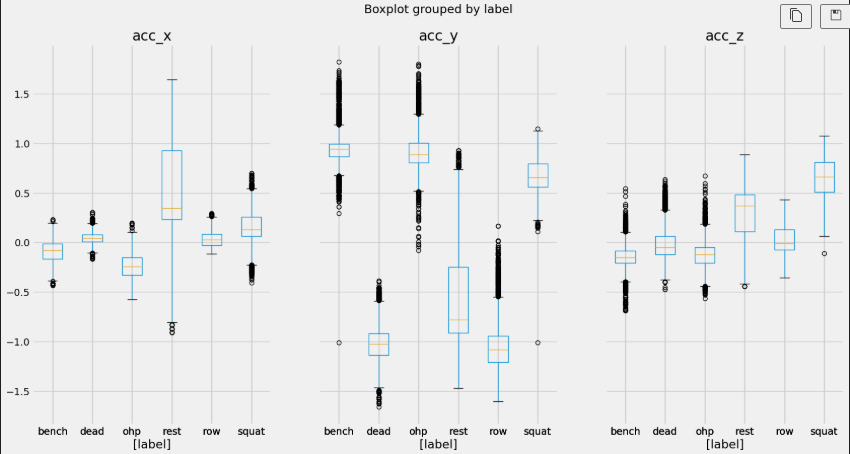
\includegraphics[width=0.95\textwidth]{figures/boxplot1.png}
\caption{Outliers values in $acc_{X Y Z}$ directions using IQR Boxplot }
\end{figure}

\begin{figure}[H]
\centering
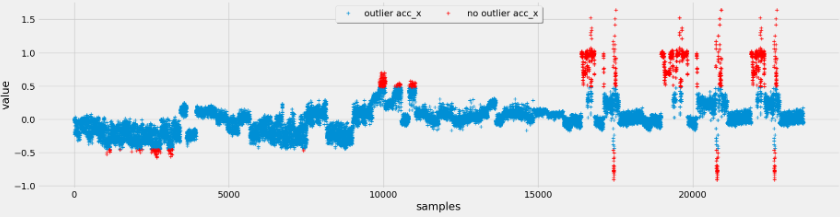
\includegraphics[width=0.95\textwidth]{figures/IQR.png}
\caption{Outliers values in $acc_{X}$ directions using IQR }
\end{figure}

\subsection{Chauvenet's Criterion}

Chauvenet's Criterion is another statistical approach used to detect outliers by considering the probability of observing a given data point in a normally distributed dataset. 
The method calculates the deviation of each observation from the mean in terms of standard deviations. 
If the probability of observing such a deviation is smaller than a predefined threshold, the value is considered an outlier.

The probability threshold is defined as:

\[
P < \frac{1}{C \times N}
\]

where:
\begin{itemize}
\item $N$ is the number of observations in the dataset
\item $C$ is a constant (commonly set to 2)
\end{itemize}

This method assumes that the data follows a normal distribution. 
Therefore, histograms and box plots were used to visually check whether the sensor data approximately follows a bell-shaped distribution before applying this method.
\begin{figure}[H]
\centering
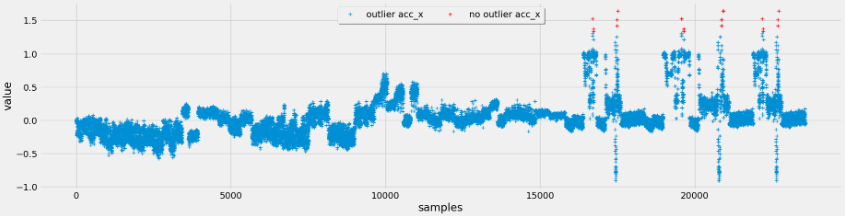
\includegraphics[width=0.95\textwidth]{figures/Chauvene_acc_x.png2.png}
\caption{ Outliers values in $acc_x$  direction  using  Chauvene }
\end{figure}

\subsection{Local Outlier Factor}

The Local Outlier Factor (LOF) is a density-based anomaly detection algorithm. 
Unlike the previous methods, LOF is a machine learning approach that identifies outliers based on the local density of data points relative to their neighbors.

The algorithm compares the density of each observation to the densities of its nearest neighbors. 
If a point has a significantly lower density than its neighbors, it is considered an outlier.

In this project, the LOF algorithm from the \texttt{scikit-learn} library was used with 20 nearest neighbors. 
Instead of analyzing individual columns separately, LOF evaluates all selected sensor features simultaneously, allowing it to detect anomalies based on the combined behavior of multiple sensors.

This approach is particularly useful for multidimensional datasets where relationships between features may reveal abnormal observations.

\begin{figure}[H]
\centering
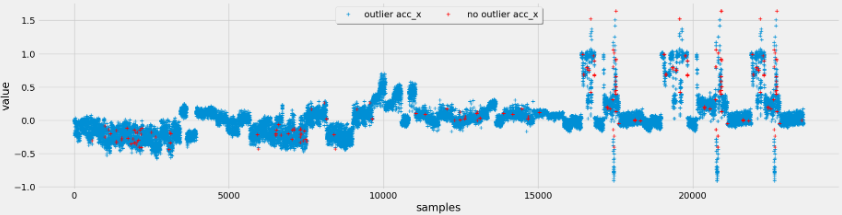
\includegraphics[width=0.95\textwidth]{figures/LOF.png}
\caption{ Outliers values in $acc_x$  direction  using  LOF }
\end{figure}

%------------------------------------------------
\section{Feature Engineering}

\subsection{Overview}

Feature engineering is the process of transforming raw sensor data into informative variables that improve the performance of machine learning models. 
Since raw accelerometer and gyroscope signals are often noisy and complex, several transformation techniques were applied to extract meaningful patterns from the motion data.

The feature engineering pipeline consisted of the following steps:

\begin{itemize}
\item Noise filtering of raw signals
\item Dimensionality reduction using Principal Component Analysis (PCA)
\item Computation of signal magnitude features
\item Extraction of temporal statistical features
\item Extraction of frequency domain features using Fourier Transform
\item Motion pattern grouping using clustering
\end{itemize}

These features help the machine learning model better distinguish between different types of barbell exercises.

\subsection{Noise Filtering}

Raw signals obtained from wearable sensors often contain high-frequency noise caused by sensor vibrations or environmental disturbances. 
To smooth the signals and retain the important motion patterns, a Butterworth low-pass filter was applied to the accelerometer and gyroscope data.

The Butterworth filter is commonly used in signal processing because it preserves the overall shape of the signal while removing rapid fluctuations.

Applying the low-pass filter results in smoother signals that better represent the underlying body movement during exercises.

\begin{figure}[H]
\centering
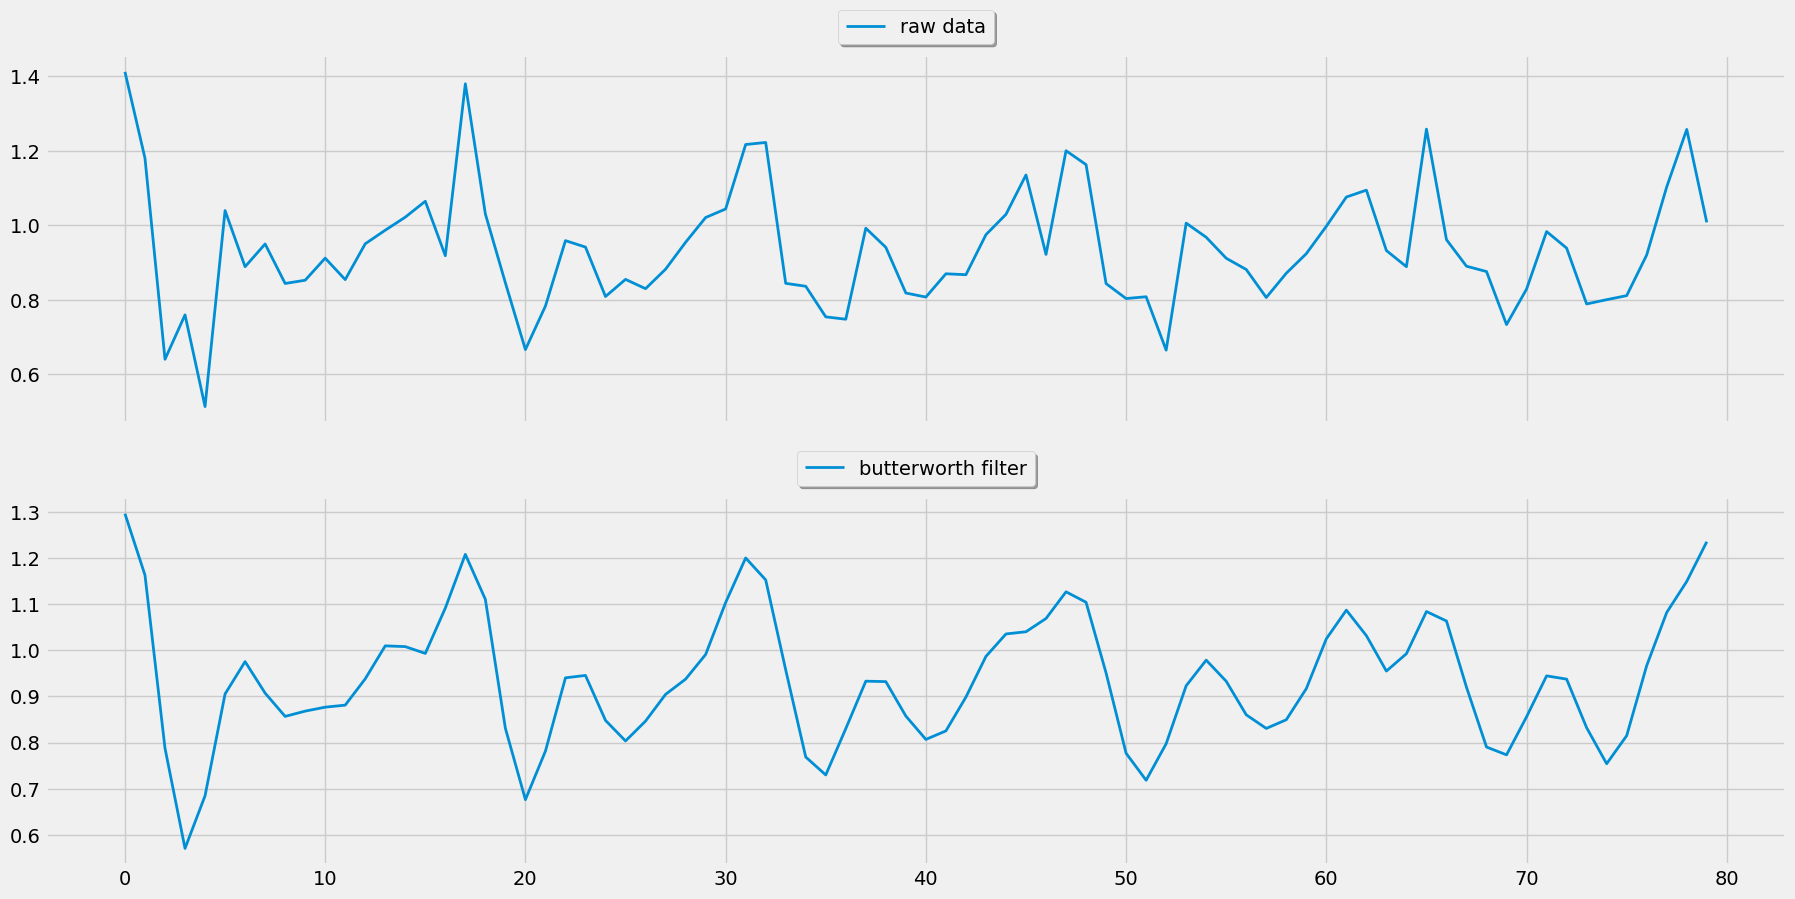
\includegraphics[width=0.9\textwidth]{figures/low_pass_filter_example.png}
\caption{Example of accelerometer signal before and after applying a Butterworth low-pass filter.}
\label{fig:lowpass}
\end{figure}



\subsection{Principal Component Analysis}

Principal Component Analysis (PCA) was applied to reduce the dimensionality of the dataset while preserving most of the important information.

Since the accelerometer and gyroscope provide multiple correlated signals (X, Y, Z axes), PCA transforms these correlated variables into a smaller number of uncorrelated components called principal components.

These components capture the most significant variance in the data and help simplify the learning process for machine learning models.

Using PCA also helps reduce noise and redundancy in the dataset.

\begin{figure}[H]
\centering
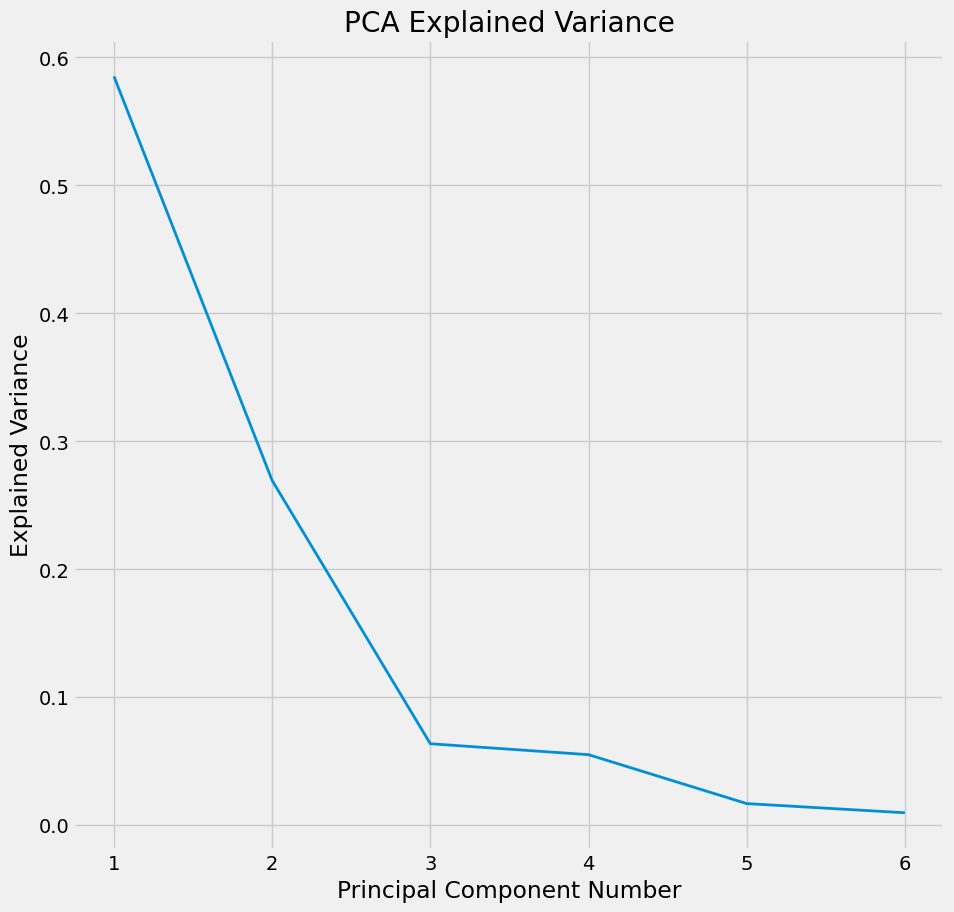
\includegraphics[width=0.75\textwidth]{figures/pca_variance_explained.png}
\caption{Explained variance ratio of principal components.}
\label{fig:pca}
\end{figure}



\subsection{Magnitude Features}

In addition to the individual axis measurements, the overall magnitude of motion was calculated for both the accelerometer and gyroscope signals.

The magnitude combines the three spatial axes into a single value representing the total movement intensity.

For the accelerometer signal, the magnitude is computed as:

\[
Acc_{mag} = \sqrt{acc_x^2 + acc_y^2 + acc_z^2}
\]

Similarly, the gyroscope magnitude is calculated as:

\[
Gyr_{mag} = \sqrt{gyr_x^2 + gyr_y^2 + gyr_z^2}
\]

These magnitude features help capture the total motion regardless of direction and are useful for distinguishing exercise types.

\begin{figure}[H]
\centering
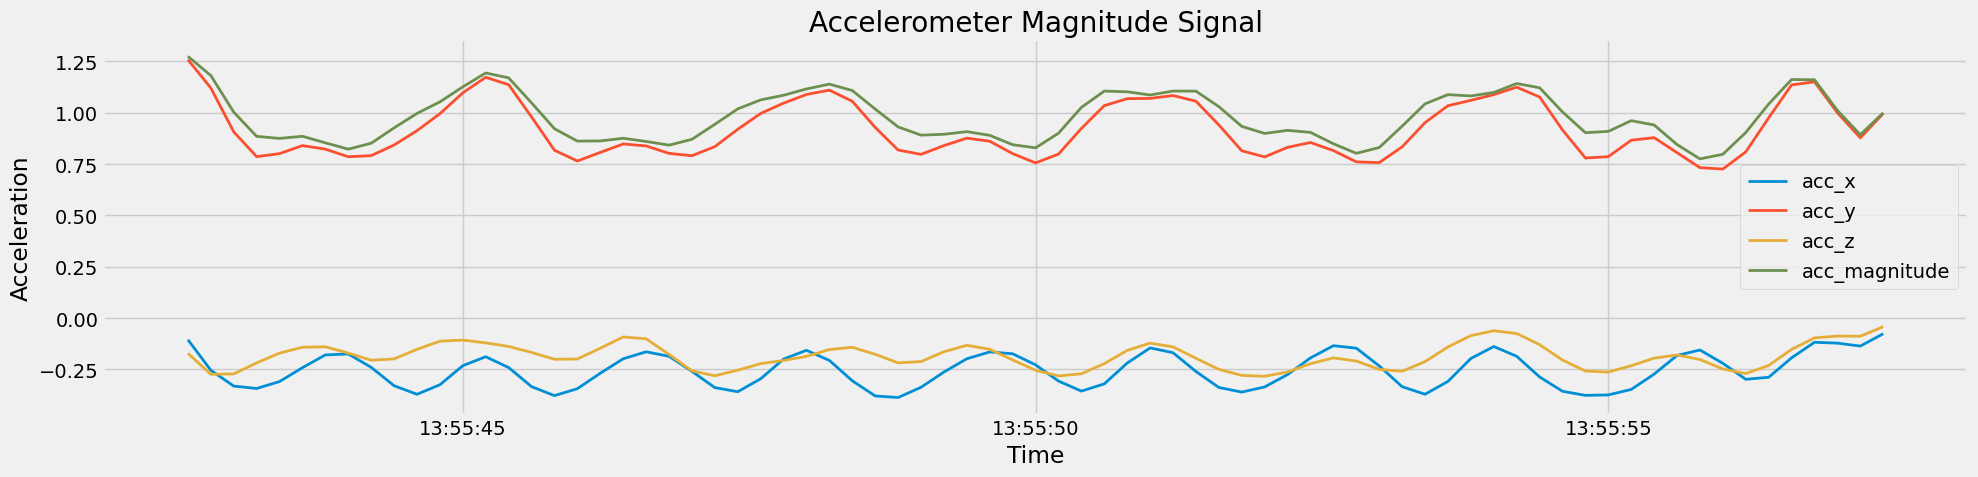
\includegraphics[width=0.85\textwidth]{figures/magnitude_signal.png}
\caption{Example magnitude signal computed from accelerometer axes.}
\label{fig:magnitude}
\end{figure}

\subsection{Temporal Features}

Temporal features were extracted using rolling windows applied to the time series signals.

A rolling window calculates statistical measures over a fixed time interval, capturing how the signal evolves over time. 
Examples of temporal features include:

\begin{itemize}
\item Rolling mean
\item Rolling standard deviation
\item Rolling minimum
\item Rolling maximum
\end{itemize}

These features capture patterns in the movement dynamics and help detect repetitive exercise motions.


\subsection{Frequency Features}

To analyze periodic patterns in exercise movements, the Discrete Fourier Transform (DFT) was applied to convert the signals from the time domain into the frequency domain.

Frequency domain features reveal dominant motion frequencies, which are particularly useful for identifying repetitive actions such as lifting repetitions.

Key frequency features include:

\begin{itemize}
\item Dominant frequency
\item Frequency energy
\item Spectral entropy
\end{itemize}

These features provide valuable information about the rhythm and periodicity of movements.

\begin{figure}[H]
\centering
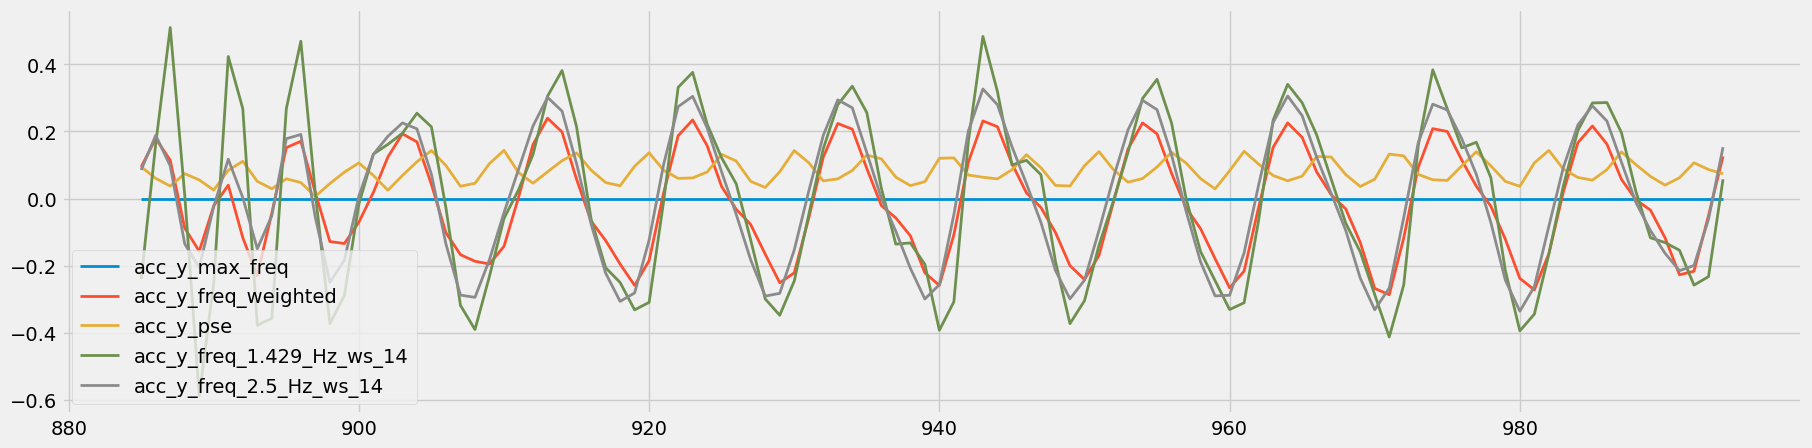
\includegraphics[width=0.85\textwidth]{figures/fourier_transform_example.png}
\caption{Frequency spectrum obtained using the Fourier Transform.}
\label{fig:fft}
\end{figure}



\subsection{Clustering Features}

Finally, clustering techniques were applied to identify groups of similar motion patterns within the dataset. 
K-means clustering was used to partition the sensor data into clusters representing different movement behaviors.

Clustering can reveal hidden structures in the motion data and help identify variations within exercises such as different lifting intensities.

The resulting cluster labels were added as additional features for the machine learning models.

\begin{figure}[H]
\centering
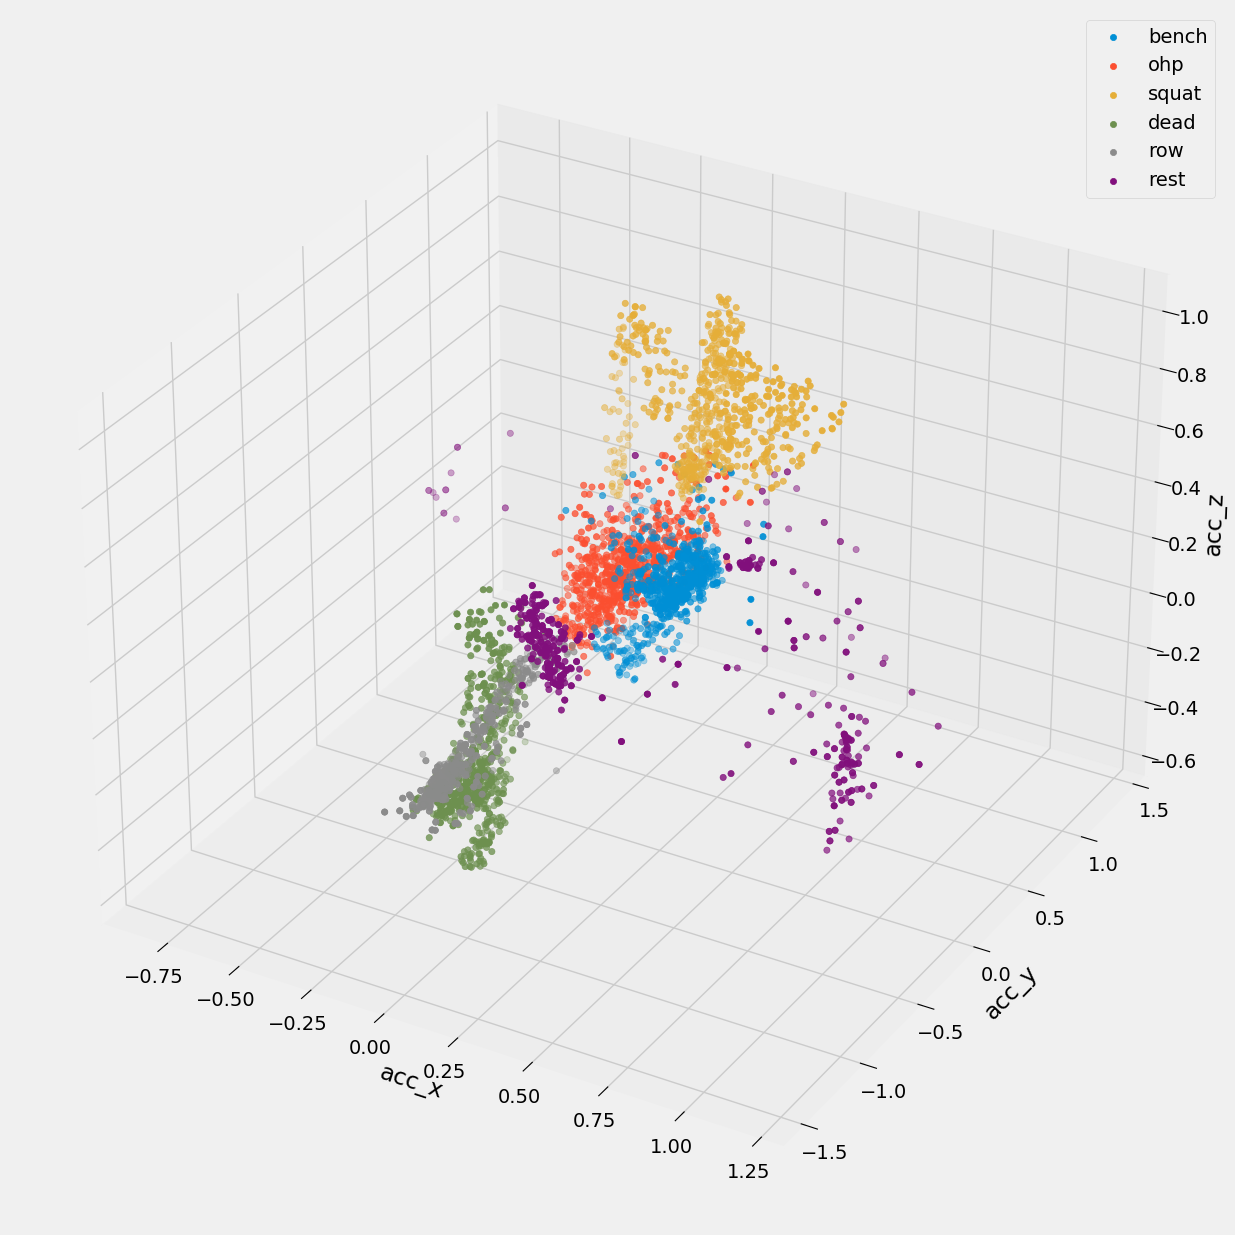
\includegraphics[width=0.8\textwidth]{figures/kmeans_clusters.png}
\caption{Example clustering of motion patterns using K-means.}
\label{fig:kmeans}
\end{figure}

%------------------------------------------------
\section{Machine Learning Models}

\subsection{Training and Testing Split}

The dataset was divided into training and testing subsets using a stratified sampling approach to preserve the class distribution of exercise labels.

First, non-relevant columns such as participant ID, category, and set number were removed. The remaining features were used as input variables, while the exercise label was used as the target variable.

The dataset was split using a 75\% training and 25\% testing ratio:

\begin{itemize}
\item Training set: used to train the models
\item Test set: used to evaluate model performance
\end{itemize}

Stratification ensured that each exercise class was equally represented in both sets.

\begin{figure}[H]
\centering
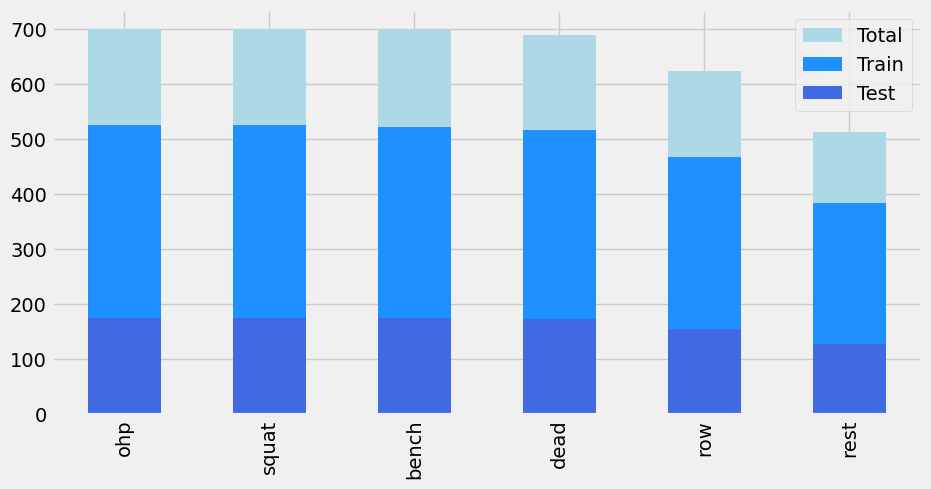
\includegraphics[width=0.8\textwidth]{figures/train_test_distribution.png}
\caption{Distribution of labels in total, training, and testing datasets.}
\label{fig:train_test}
\end{figure}


\subsection{Feature Selection}

Feature selection was performed using forward feature selection with a simple decision tree model. This method incrementally selects features that improve classification accuracy.

The process evaluated up to 10 features and ranked them based on their contribution to model performance.

The final selected features were mainly derived from frequency domain features, indicating that frequency characteristics are highly informative for distinguishing exercise types.

\begin{figure}[H]
\centering
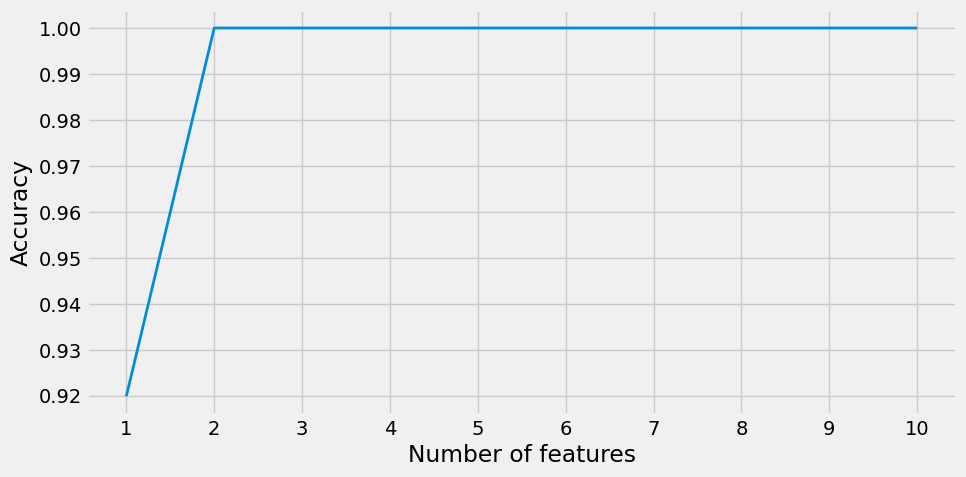
\includegraphics[width=0.7\textwidth]{figures/feature_selection.png}
\caption{Forward feature selection showing accuracy improvement as features are added.}
\label{fig:feature_selection}
\end{figure}


\subsection{Models Used}

Several machine learning models were trained and evaluated on different feature sets.

\subsubsection{Naive Bayes}

Naive Bayes is a probabilistic classifier based on Bayes' theorem. It assumes independence between features and provides a simple yet effective baseline model.

\subsubsection{Support Vector Machine}

Support Vector Machines (SVM) are powerful classifiers that aim to find the optimal hyperplane that separates classes in high-dimensional space. Although not explicitly implemented in the final pipeline, similar deterministic models such as K-Nearest Neighbors and Decision Trees were evaluated.

\subsubsection{Random Forest}

Random Forest is an ensemble learning method that constructs multiple decision trees and combines their predictions. It is robust to noise and performs well on complex datasets.

\subsubsection{Neural Network}

A feedforward neural network was used as a non-linear model capable of capturing complex relationships in the data. Due to its stochastic nature, multiple runs were averaged to obtain stable performance estimates.

\subsection{Hyperparameter Tuning}

Hyperparameter tuning was performed using grid search for several models, including Random Forest, K-Nearest Neighbors, and Decision Trees.

Grid search evaluates different parameter combinations and selects the configuration that maximizes model performance on the validation set.

For non-deterministic models such as neural networks and random forests, multiple iterations were performed and averaged to ensure reliable results.

\subsection{Model Evaluation}

Models were evaluated using classification accuracy on the test dataset. Additionally, confusion matrices were used to analyze the classification performance for each exercise class.

A grouped bar plot was created to compare the performance of different models across multiple feature sets.

\begin{figure}[H]
\centering
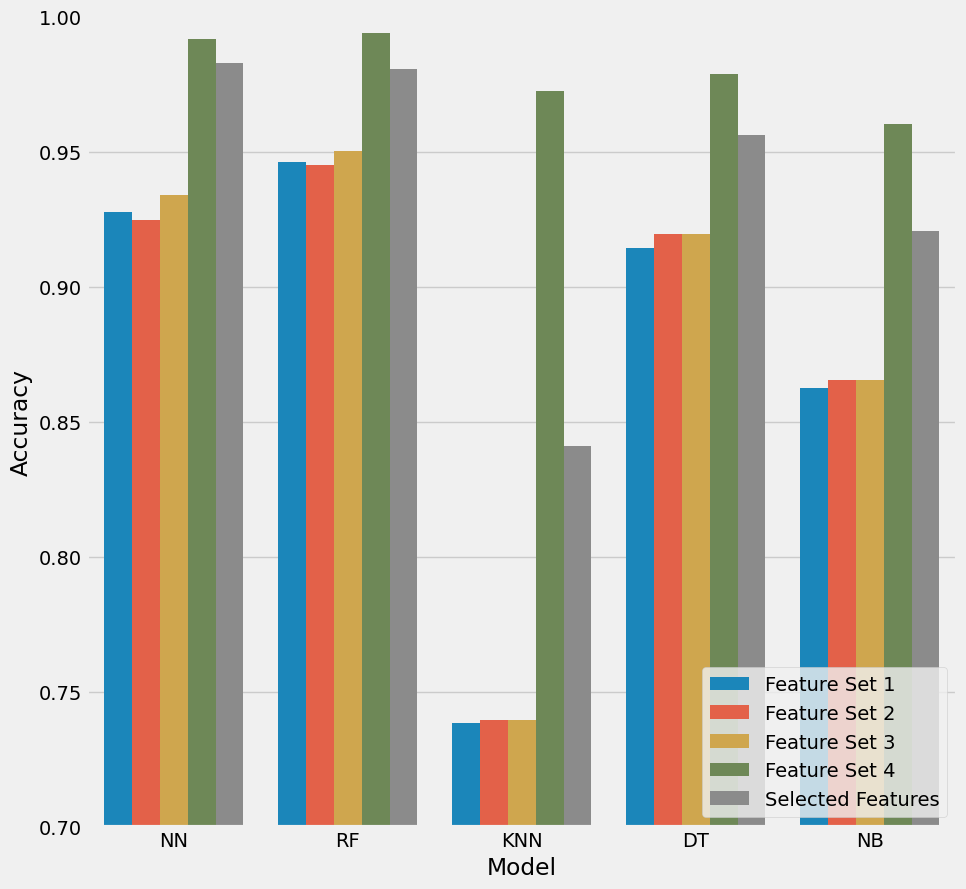
\includegraphics[width=0.65\textwidth]{figures/model_comparison.png}
\caption{Comparison of model accuracy across different feature sets.}
\label{fig:model_comparison}
\end{figure}


The Random Forest model achieved the best overall performance and was selected as the final model.

\subsubsection{Confusion Matrix}

To further evaluate the model, a confusion matrix was generated to visualize the classification results.

\begin{figure}[H]
\centering
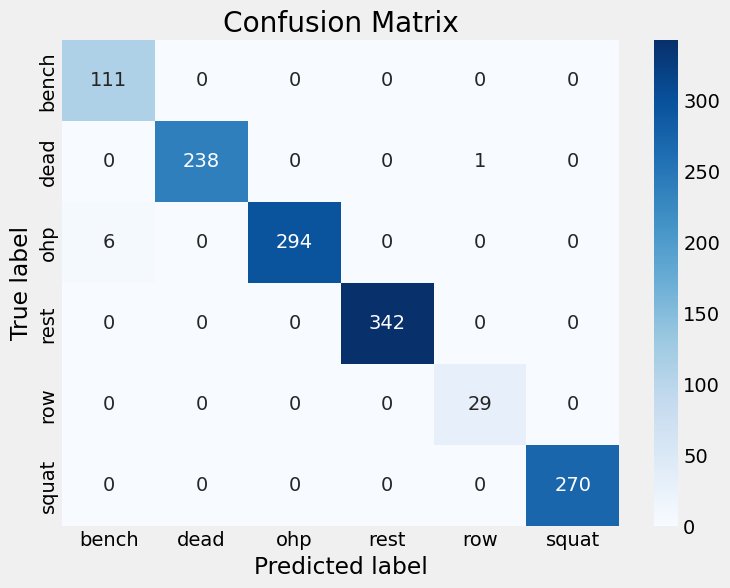
\includegraphics[width=0.7\textwidth]{figures/confusion_matrix.png}
\caption{Confusion matrix of the best performing model.}
\label{fig:confusion_matrix}
\end{figure}


\subsubsection{Generalization Across Participants}

To evaluate model robustness, an additional experiment was conducted where the model was trained on data from all participants except one and tested on the unseen participant.

This approach simulates real-world conditions where the model must generalize to new users.

The Random Forest model maintained strong performance, demonstrating its ability to generalize across different individuals performing the same exercises.

\begin{table}[H]
\centering
\begin{tabular}{cccccc}
\toprule
Model & FS1 & FS2 & FS3 & FS4 & Selected \\
\midrule
Neural Network & 0.931 & 0.928 & 0.924 & \textbf{0.987} & 0.977 \\
Random Forest  & 0.951 & 0.950 & 0.952 & \textbf{0.995} & 0.980 \\
KNN            & 0.738 & 0.739 & 0.739 & \textbf{0.973} & 0.841 \\
Decision Tree  & 0.909 & 0.910 & 0.919 & \textbf{0.985} & 0.961 \\
Naive Bayes    & 0.863 & 0.866 & 0.866 & \textbf{0.958} & 0.921 \\
\bottomrule
\end{tabular}
\caption{Model accuracy comparison across different feature sets}
\end{table}

The results clearly show that Feature Set 4, which includes all engineered features (temporal, frequency, and clustering), provides the highest accuracy across all models. 

Random Forest and Neural Network achieved the best performance with an accuracy close to 99\%, demonstrating their ability to capture complex patterns in the sensor data.

KNN performed poorly on basic feature sets but significantly improved when advanced features were included, highlighting the importance of feature engineering.

Overall, feature engineering had a greater impact on performance than the choice of model itself.
%------------------------------------------------
\section{Repetition Counting}

\subsection{Exercise Pattern Analysis}

The motion sensor signals exhibit periodic patterns that correspond to individual exercise repetitions. By visualizing accelerometer and gyroscope signals for a single set, it is possible to observe clear repeating peaks and valleys that represent the movement cycles of each repetition.

To better understand these patterns, multiple signals such as \texttt{acc\_x}, \texttt{acc\_y}, \texttt{acc\_z}, and their magnitude \texttt{acc\_r} were plotted. Similarly, gyroscope signals were analyzed.

\begin{figure}[H]
\centering
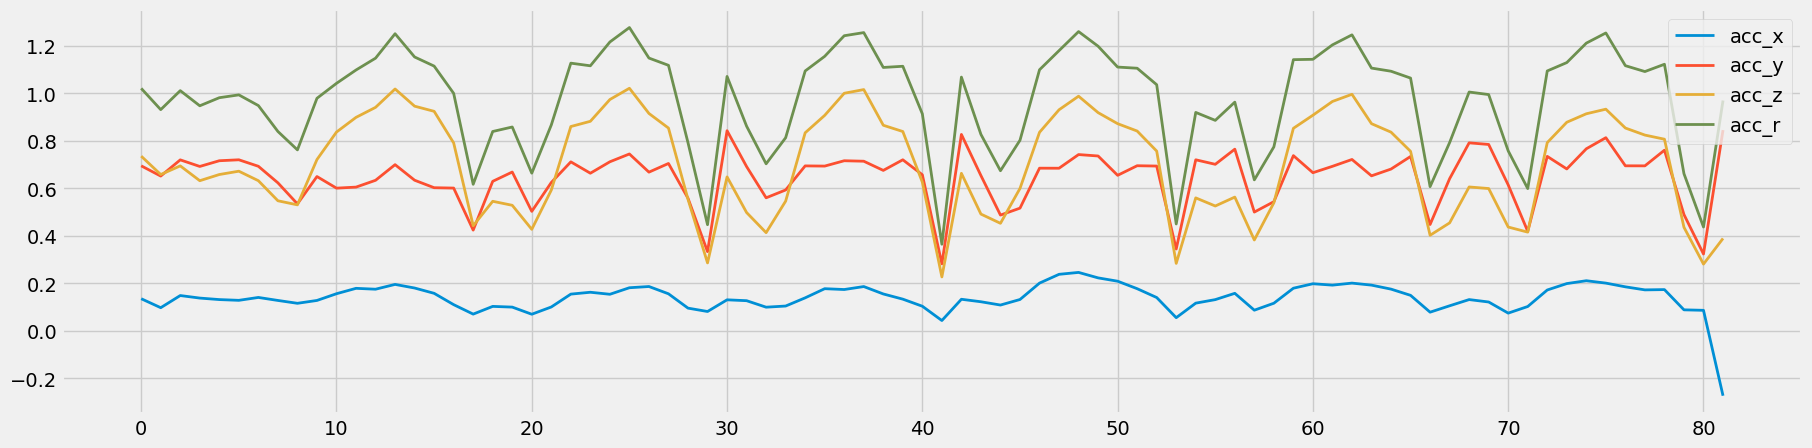
\includegraphics[width=0.9\linewidth]{figures/exercise_signal_pattern.png}
\caption{Example of raw sensor signals showing repetitive patterns during an exercise set}
\end{figure}


\vspace{0.5cm}

\subsection{Signal Filtering}

Raw sensor data contains noise that makes it difficult to clearly identify repetitions. To address this, a Butterworth low-pass filter was applied to smooth the signals and highlight the underlying motion pattern.

The filter was applied using a sampling frequency of 5 Hz and different cutoff frequencies depending on the exercise type. For example:
\begin{itemize}
\item Bench press: cutoff = 0.4 Hz
\item Squat: cutoff = 0.35 Hz
\item Row: cutoff = 0.65 Hz
\end{itemize}

\begin{figure}[H]
\centering
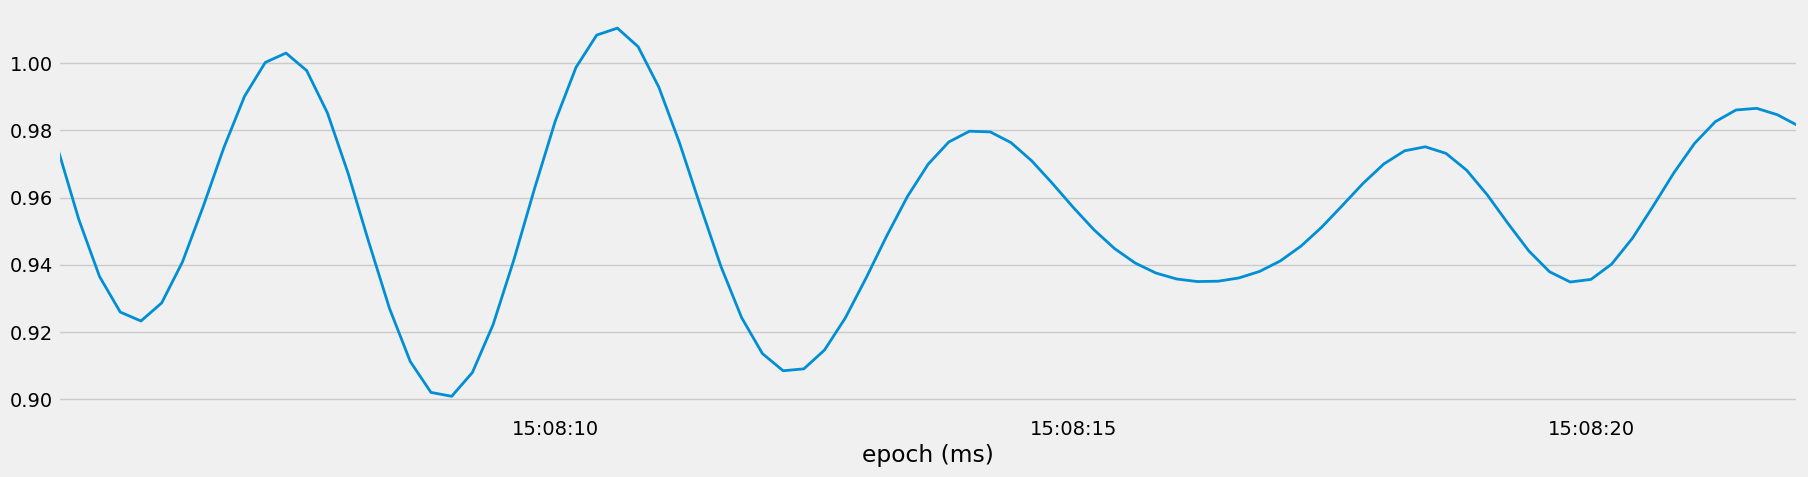
\includegraphics[width=0.9\linewidth]{figures/lowpass_repetition_signal.png}
\caption{Comparison between raw signal and filtered signal showing clearer repetition patterns}
\end{figure}

\vspace{0.5cm}

\subsection{Repetition Counting Algorithm}

A custom algorithm was developed to automatically count repetitions based on the filtered signal.

The main steps of the algorithm are:
\begin{enumerate}
\item Apply a low-pass filter to the selected signal (e.g., \texttt{acc\_r} or \texttt{gyr\_x})
\item Detect local maxima (peaks) using \texttt{argrelextrema}
\item Count the number of peaks, where each peak represents one repetition
\end{enumerate}

The implementation is shown below:

\begin{lstlisting}
def count_reps(dataset, cutoff=0.4, order=10, column="acc_r"): 
    data = LowPass.low_pass_filter( 
        dataset, col=column, sampling_frequency=fs, cutoff_frequency=cutoff, order=order 
    ) 
     
    indexes = argrelextrema(data[column + "_lowpass"].values, np.greater) 
    peaks = data.iloc[indexes] 
     
    return len(peaks) 
\end{lstlisting}

Different exercises required different configurations:
\begin{itemize}
\item Squat: lower cutoff frequency (0.35 Hz)
\item Row: used gyroscope signal (\texttt{gyr\_x}) instead of accelerometer
\item Other exercises: used \texttt{acc\_r} signal
\end{itemize}

\begin{figure}[H]
\centering
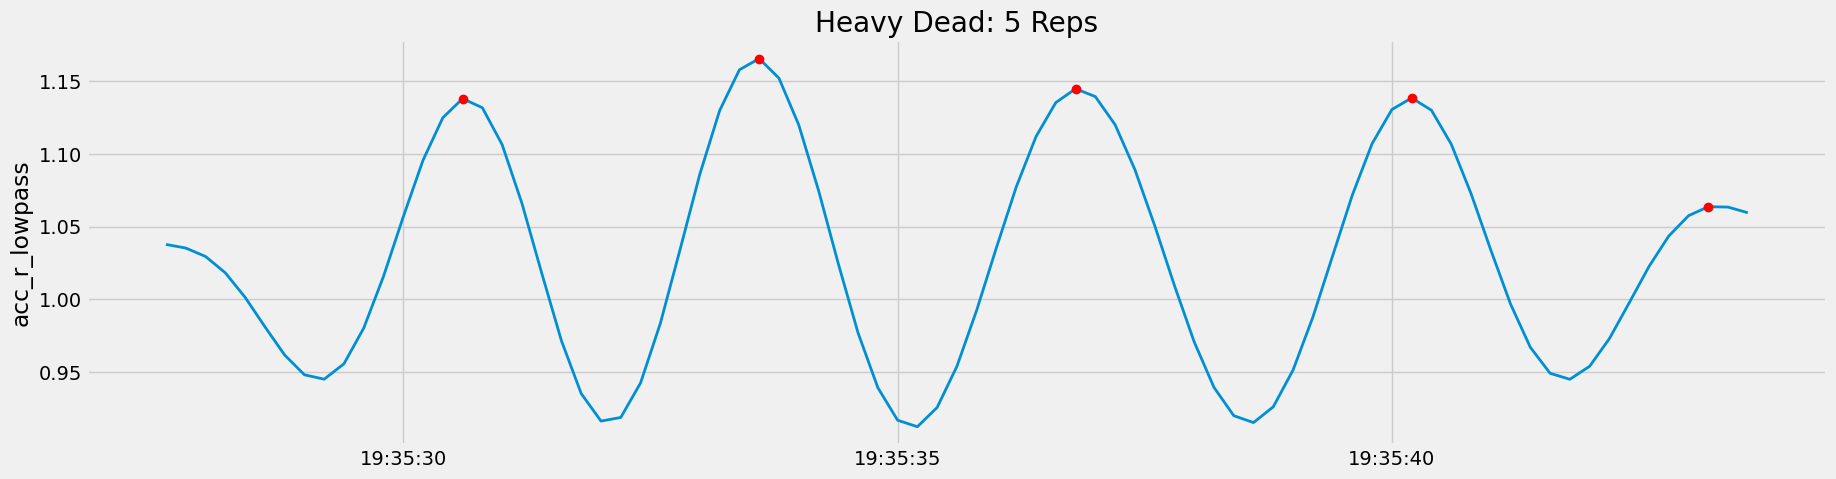
\includegraphics[width=0.9\linewidth]{figures/repetition_peaks.png}
\caption{Detected peaks corresponding to repetitions in the filtered signal}
\end{figure}

\vspace{0.5cm}

\subsection{Evaluation}

To evaluate the performance of the repetition counting algorithm, a benchmark dataset was created. The ground truth number of repetitions was defined based on the exercise intensity:
\begin{itemize}
\item Heavy sets: 5 repetitions
\item Medium/light sets: 10 repetitions
\end{itemize}

The predicted repetitions were compared against the ground truth using Mean Absolute Error (MAE):

\begin{lstlisting}
error = mean_absolute_error(rep_df["reps"], rep_df["reps_pred"]).round(2)
\end{lstlisting}

Additionally, the average predicted and actual repetitions per exercise were visualized:

\begin{figure}[H]
\centering
    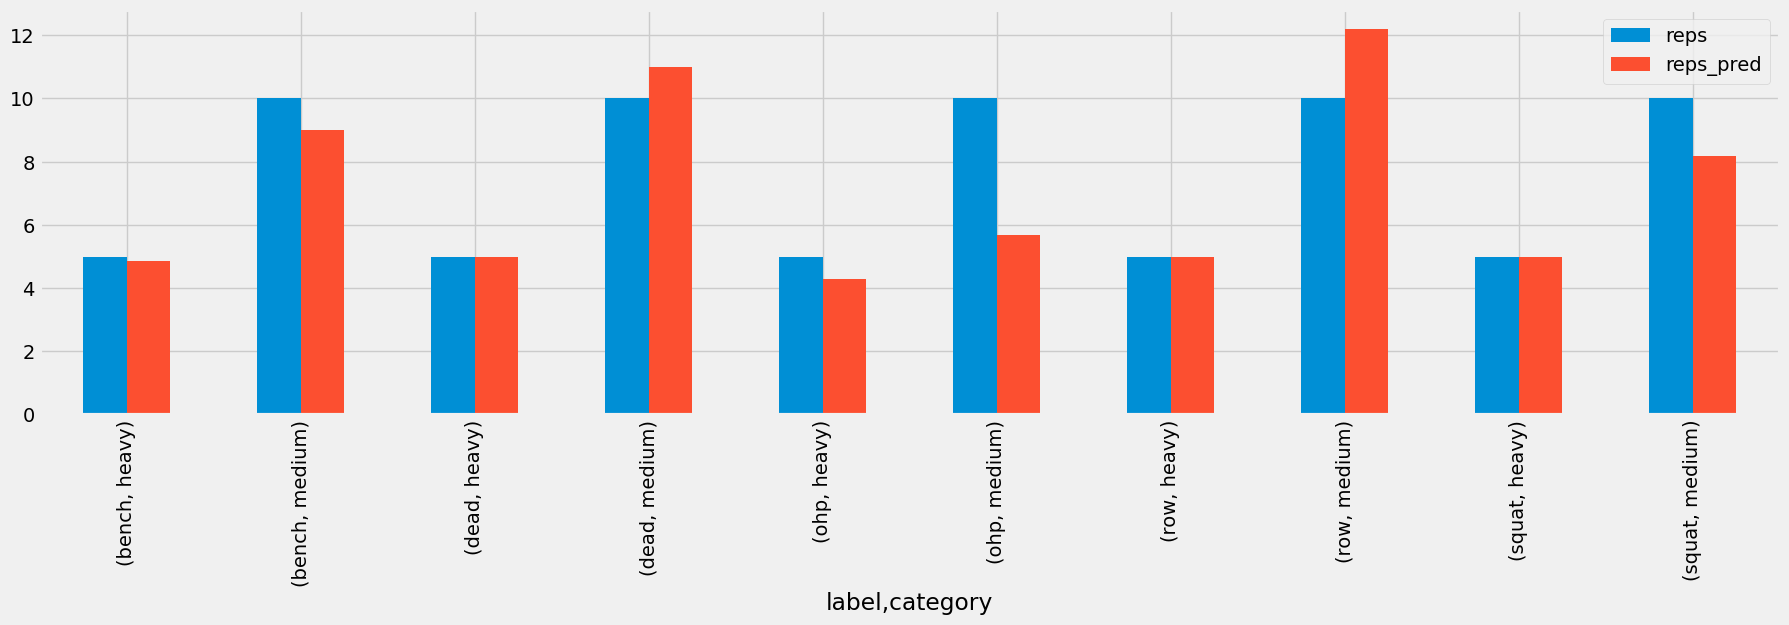
\includegraphics[width=0.9\linewidth]{figures/repetition_evaluation.png}
\caption{Comparison between actual and predicted repetitions across exercises}
\end{figure}


Bar chart from:
\begin{lstlisting}
rep_df.groupby(["label", "category"])["reps", "reps_pred"].mean().plot.bar()
\end{lstlisting}

The results showed that the algorithm is capable of accurately estimating repetitions for most exercises, although small deviations may occur due to noise, variation in movement speed, and differences between participants.

%------------------------------------------------
\section{Results and Discussion}

\subsection{Best Model Performance}

The Random Forest model achieved the highest performance among all tested models, reaching an accuracy close to 99\% when using the full feature set (Feature Set 4). Neural Networks also demonstrated competitive performance, indicating that complex models benefit significantly from the engineered features.

\subsection{Observations}

The results highlight the importance of feature engineering in this project. Features extracted from temporal, frequency, and clustering techniques significantly improved classification performance compared to using raw sensor data alone.

Additionally, different exercises exhibited distinct motion patterns in both accelerometer and gyroscope signals, which made them separable using machine learning models.

\subsection{Limitations}

\begin{itemize}
\item Limited number of participants (only a small group was included)
\item Dataset size is relatively small for robust generalization
\item Variability in sensor placement may affect signal consistency
\end{itemize}

%------------------------------------------------
\section{Conclusion}

\subsection{Summary}

This project demonstrated how machine learning techniques can be applied to classify barbell exercises using wearable sensor data. Starting from raw accelerometer and gyroscope signals, the pipeline included data preprocessing, feature engineering, model training, and evaluation.

The results showed that combining advanced feature engineering with powerful models such as Random Forest leads to highly accurate classification performance.

The full implementation of the project is available at:  
\url{https://github.com/M0hamed-Eid/FitnessTracker.git}

\subsection{Future Work}

Future improvements for this project include:

\begin{itemize}
\item Collecting more data from a larger and more diverse group of participants
\item Deploying the model as a real-time application (e.g., web or mobile app)
\item Improving robustness for different sensor placements and environments
\end{itemize}

%------------------------------------------------
\section{References}

\begin{itemize}
\item Hoogendoorn, M., \& Funk, B. (2018). \textit{Machine Learning for the Quantified Self}.
\item ML4QS Project Website: \url{https://ml4qs.org}
\item MetaMotion Sensor: \url{https://mbientlab.com/metamotions/}
\end{itemize}

%------------------------------------------------
\end{document}

\begin{figure}[H]
\centering
\includegraphics[width=0.95\textwidth]{figures/}
\caption{}
\end{figure}